\documentclass[12pt,twoside]{article}

\def\refname{\underline{\normalsize References}}
\def\title#1{\begin{center}{\large\bf #1}\end{center}}

\renewcommand{\author}[2]{\noindent\underbar{#1}\\#2\\}
\newcommand{\coauthor}[2]{\noindent\underbar{#1}\\#2\\}

\usepackage[paperwidth=20.5cm,paperheight=29.7cm,width=18cm,height=26.5cm,top=24mm,left=14mm,headsep=11mm]{geometry}

\usepackage{graphicx}

\usepackage{amsmath,bm}

\pagestyle{myheadings} \markboth{DAYS on DIFFRACTION 2016}{DAYS on DIFFRACTION 2016}

\begin{document}

\title{Resonant states for quantum ring with two infinite leads}

\author{\textbf{Gerasimov D.A.}, Popov I.Y., Popov A.I.} % presenting author is marked out by \textbf 
{Department of Higher Mathematics, ITMO University, Saint Petersburg 197101,
Russia\\ e-mail: {\tt karlicoss@gmail.com, popov1955@gmail.com, popov239@gmail.com} }

% for name index
\index{Gerasimov, D.A.} 
\index{Popov, I.U.}
\index{Popov, A.I.}


% TODO move up?
\newcommand\abs[1]{\left|#1\right|}

% Text:

Quantum graph is a widely used model of nanosystem [1-4] TODO. If the graph $\Gamma$ consists of finite number of edges and all edges have finite lengths then the Hamiltonian has purely discrete spectrum. The system of eigenfunctions is complete in $L_2(\Gamma)$. If the graph contains semi-infinite edges, one has non-empty continuous spectrum and resonances generated by the eigenvalues of the initial Hamiltonian of finite graph. For many applications, it is important to know a space in which the resonant states form a complete system. In the present paper we determine this space for a graph with two infinite leads and one loop using Sz.-Nagy model [5].

Due to the symmetry of the problem, scattering matrix $S$ takes the form TODO MATRIX, and solving the system of equations, we obtain:
\[
\det S = \frac{}{}
\]

We establish the completeness of the resonant states in the space of square integrable functions on the ring. To show this, we have to prove that $S$ is a Blaschke-Potapov product [6], that is,

\[
\lim\limits_{r \to 1 - 0} \int\limits_{L_r} \log  \abs{\det S(z)} \frac{dz}{(z - 1)^2} = 0 ,
\]

where $L_r$ is the image of the curve $\abs{\xi} = r$ ($r < 1$) under the map $z = i \frac{1 + \xi}{1 - \xi}$. Substituting $\det S$, which we calculated above, and estimating the integral, one obtains the desired result.


\medskip
\centerline{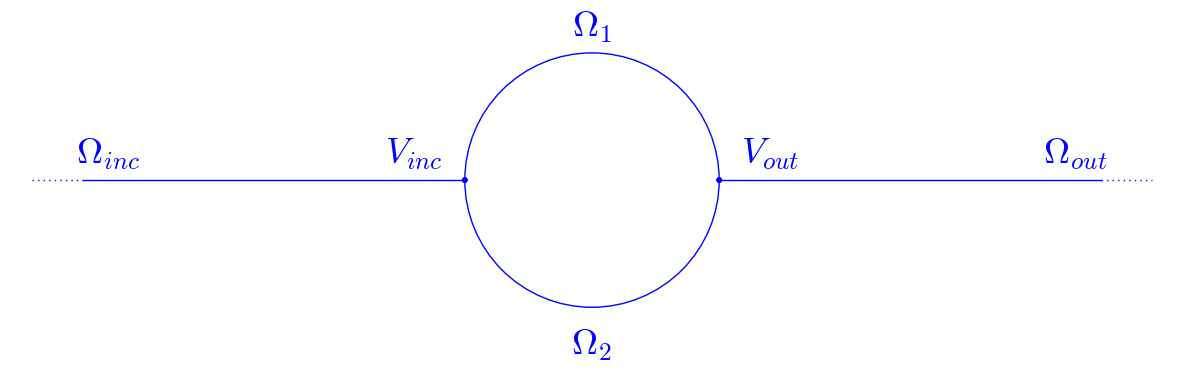
\includegraphics[width=120mm]{graph.png}}
\medskip

{\narrower\noindent \textbf{Fig.~1:}
Quantum graph $\Gamma$ consisting of edges $\Omega_{inc}, \Omega_{out}, \Omega_1, \Omega_2$. $\Omega_1$ and $\Omega_2$ represend the 1D ring connected to lead $\Omega_{inc}$ via the vertex $V_{inc}$ and to lead $\Omega_{out}$ via $V_{out}$.
\par}

\medskip


This work was partially financially supported by the Government of the Russian Federation (grant 074-U01), by Ministry of Science and Education of the Russian Federation (GOSZADANIE 2014/190, Projects No 14.Z50.31.0031 and No. 1.754.2014/K), by grant MK-5001.2015.1 of the President of the Russian Federation and DFG Grant NE~1439/3-1.


TODO COLOR
TODO WIDTH?
TODO CAN IT BE PNG?


%\centerline{\textbf{Fig. 1:} Text of short caption.}


\begin{thebibliography}{9}

\bibitem{1} A. Author, B. Author, \textit{Some good book}, Some University Press, Some City
(2010).

\bibitem{2} C. Author, \textit{Journal of Something}, \textbf{90}, 34--42 (2003).

\end{thebibliography}

\end{document}
